\section{Extracting \mt}\label{sec:ext_mt}
Extracting \mt consists of two main steps. Initially, a local orientation direction (represented as a unit vector) is computed at each grid location.
Next, we compute a coarse set of poly-cylinders called \mt which traverses the data constrained by the local orientation directions. Sec.~\ref{subsec:reliable_hessian} describes the procedure to generate Reliable Hessians. Sec.~\ref{subsec:mt_properties}  describes the \mt and their properties. Sec.~\ref{subsec:mt_generation} details the creation of MetaTracts.
\subsection{Computing Reliable Hessians}\label{subsec:reliable_hessian} 
The objective of this step is to associate each grid location with a unit vector which represents the orientation in the local neighborhood and a real value [0,1] that represents a measure of reliability of the orientation calculated at the grid location. A reliability score of 0 means the local orientation is not credible and a score of 1 means the local orientation is noisy.
The input to this stage is the original scalar data, which is an uniform lattice grid in $\mathbb{R}^3$. We approximate the local orientation  by eigenvalue analysis of the Hessian matrix applied locally to each voxel.
The Hessian matrix captures the local second-order structures inherent in the intensity (scalar values at grid vertex) variations around each grid location.
The eigen decomposition of the Hessian matrix gives the eigenvectors which represent the local curvature of the image. The eigenvector corresponding the smallest eigenvalue gives the direction along which the curvature is smallest. This direction also termed as the principal direction, coincides with the direction of the tubular structure. 


Frangi et al.~\cite{Frangi1998} introduced a process that searches for geometric structures which are tubular. They defined 
a ``vesselnes" criterion based on the geometric ratios of the second order ellipsoid given by the local Hessian matrix.
In order to determine reliable Hessians, we compute the \textit{same} metric. We include their work here for completeness and direct the reader to~\cite{Frangi1998} for details. Let $\lambda_{K}$ be the eigenvalue with the $K^{th}$ smallest magnitude. Here, $|{\lambda}_{1}| \leq| {\lambda}_{2}|\leq| {\lambda}_{3}| $ are the eigenvalues of the Hessian matrix. Specifically, a pixel belonging to a vessel region will have small $\lambda_{1}$ ($|\lambda_{1}|\approx 0$) and $\lambda_{2}$, $\lambda_{3}$ of large magnitude and of equal sign ($|\lambda_{1}| \ll |\lambda_{2}|$ and $|\lambda_{2}|\approx |\lambda_{3}|$). The sign indicates if the vessel is bright in a dark background or dark in a bright background. In our case the individual fibers are bright ($\lambda_2,\lambda_3 < 0$). The following measures are defined in~\cite{Frangi1998}.  
\begin{equation}\label{RA}
\mathcal{R_{A}}=\frac{\textrm{Largest  Cross Section}\big/ \pi}{{\textrm{Largest Axis Semi-length}}^{2}}=\frac{|\lambda_{2}|}{|\lambda_{3}|}
\end{equation}
\begin{equation}\label{RB}
\mathcal{R_{B}}=\frac{\textrm{Volume}\big/ (4\pi \big/ 3)}{{(\textrm{Largest Cross Section Area}\big/ \pi)}^{\frac{3}{2}}}=\frac{|\lambda_{1}|}{\sqrt{|\lambda_{2}\lambda_{3}|}}
\end{equation}
In Equation~\ref{RB}, $\mathcal{R_{B}}$ provides a measure of deviation from a blob like structure while in Equation~\ref{RA}, $\mathcal{R_{A}}$ distinguishes between plate-like and line-like structure. Grey-scale variations and close proximity of the fibers in our data make the Hessians computed at each voxels susceptible to errors. Thus, we compute reliable Hessians ($R_H$) to determine which locations in the volume provide reliable local orientation. 
$$
R_{H} = \left\{ \begin{array}{ccc}
0 & \mbox{ if $\lambda_{2}>0$ or $\lambda_{3}>0$} \\
(1-e^{\frac{\mathcal{-R_{A}}^{2}}{2\alpha^{2}}})
(e^{\frac{\mathcal{-R_{B}}^{2}}{2\beta^{2}}}) (1-e^{\frac{-s^2}{2c^2}}) &\mbox{ otherwise}
\end{array} \right.
$$
Variable $s$ is the Frobenius norm of the Hessian matrix. The value of $(1-e^{\frac{-s^2}{2c^2}})$ will be low in regions with no structure. The utility of the vesselness is a little different in our framework than in the work of Frangi et al.~\cite{Frangi1998}.
First, vesselness in biology is computed for different scales because the vessels can be of different sizes. In our case, usually the widths of individual fibers are known a priori.
Secondly, we do not have clear tubular structures embedded in a dark contrast matrix such as in blood vessels.
Instead, we are trying to associate each grid location  with a probable orientation based on its local second order structure. The $R_{H}$ is interpreted as a reliability measure of the local orientation.
Grid locations where the $R_{H}$ is above a cutoff threshold are marked as regions with reliable orientations (see Sec.~\ref{sec:param_choices}).

\begin{figure}[tb]
\centering
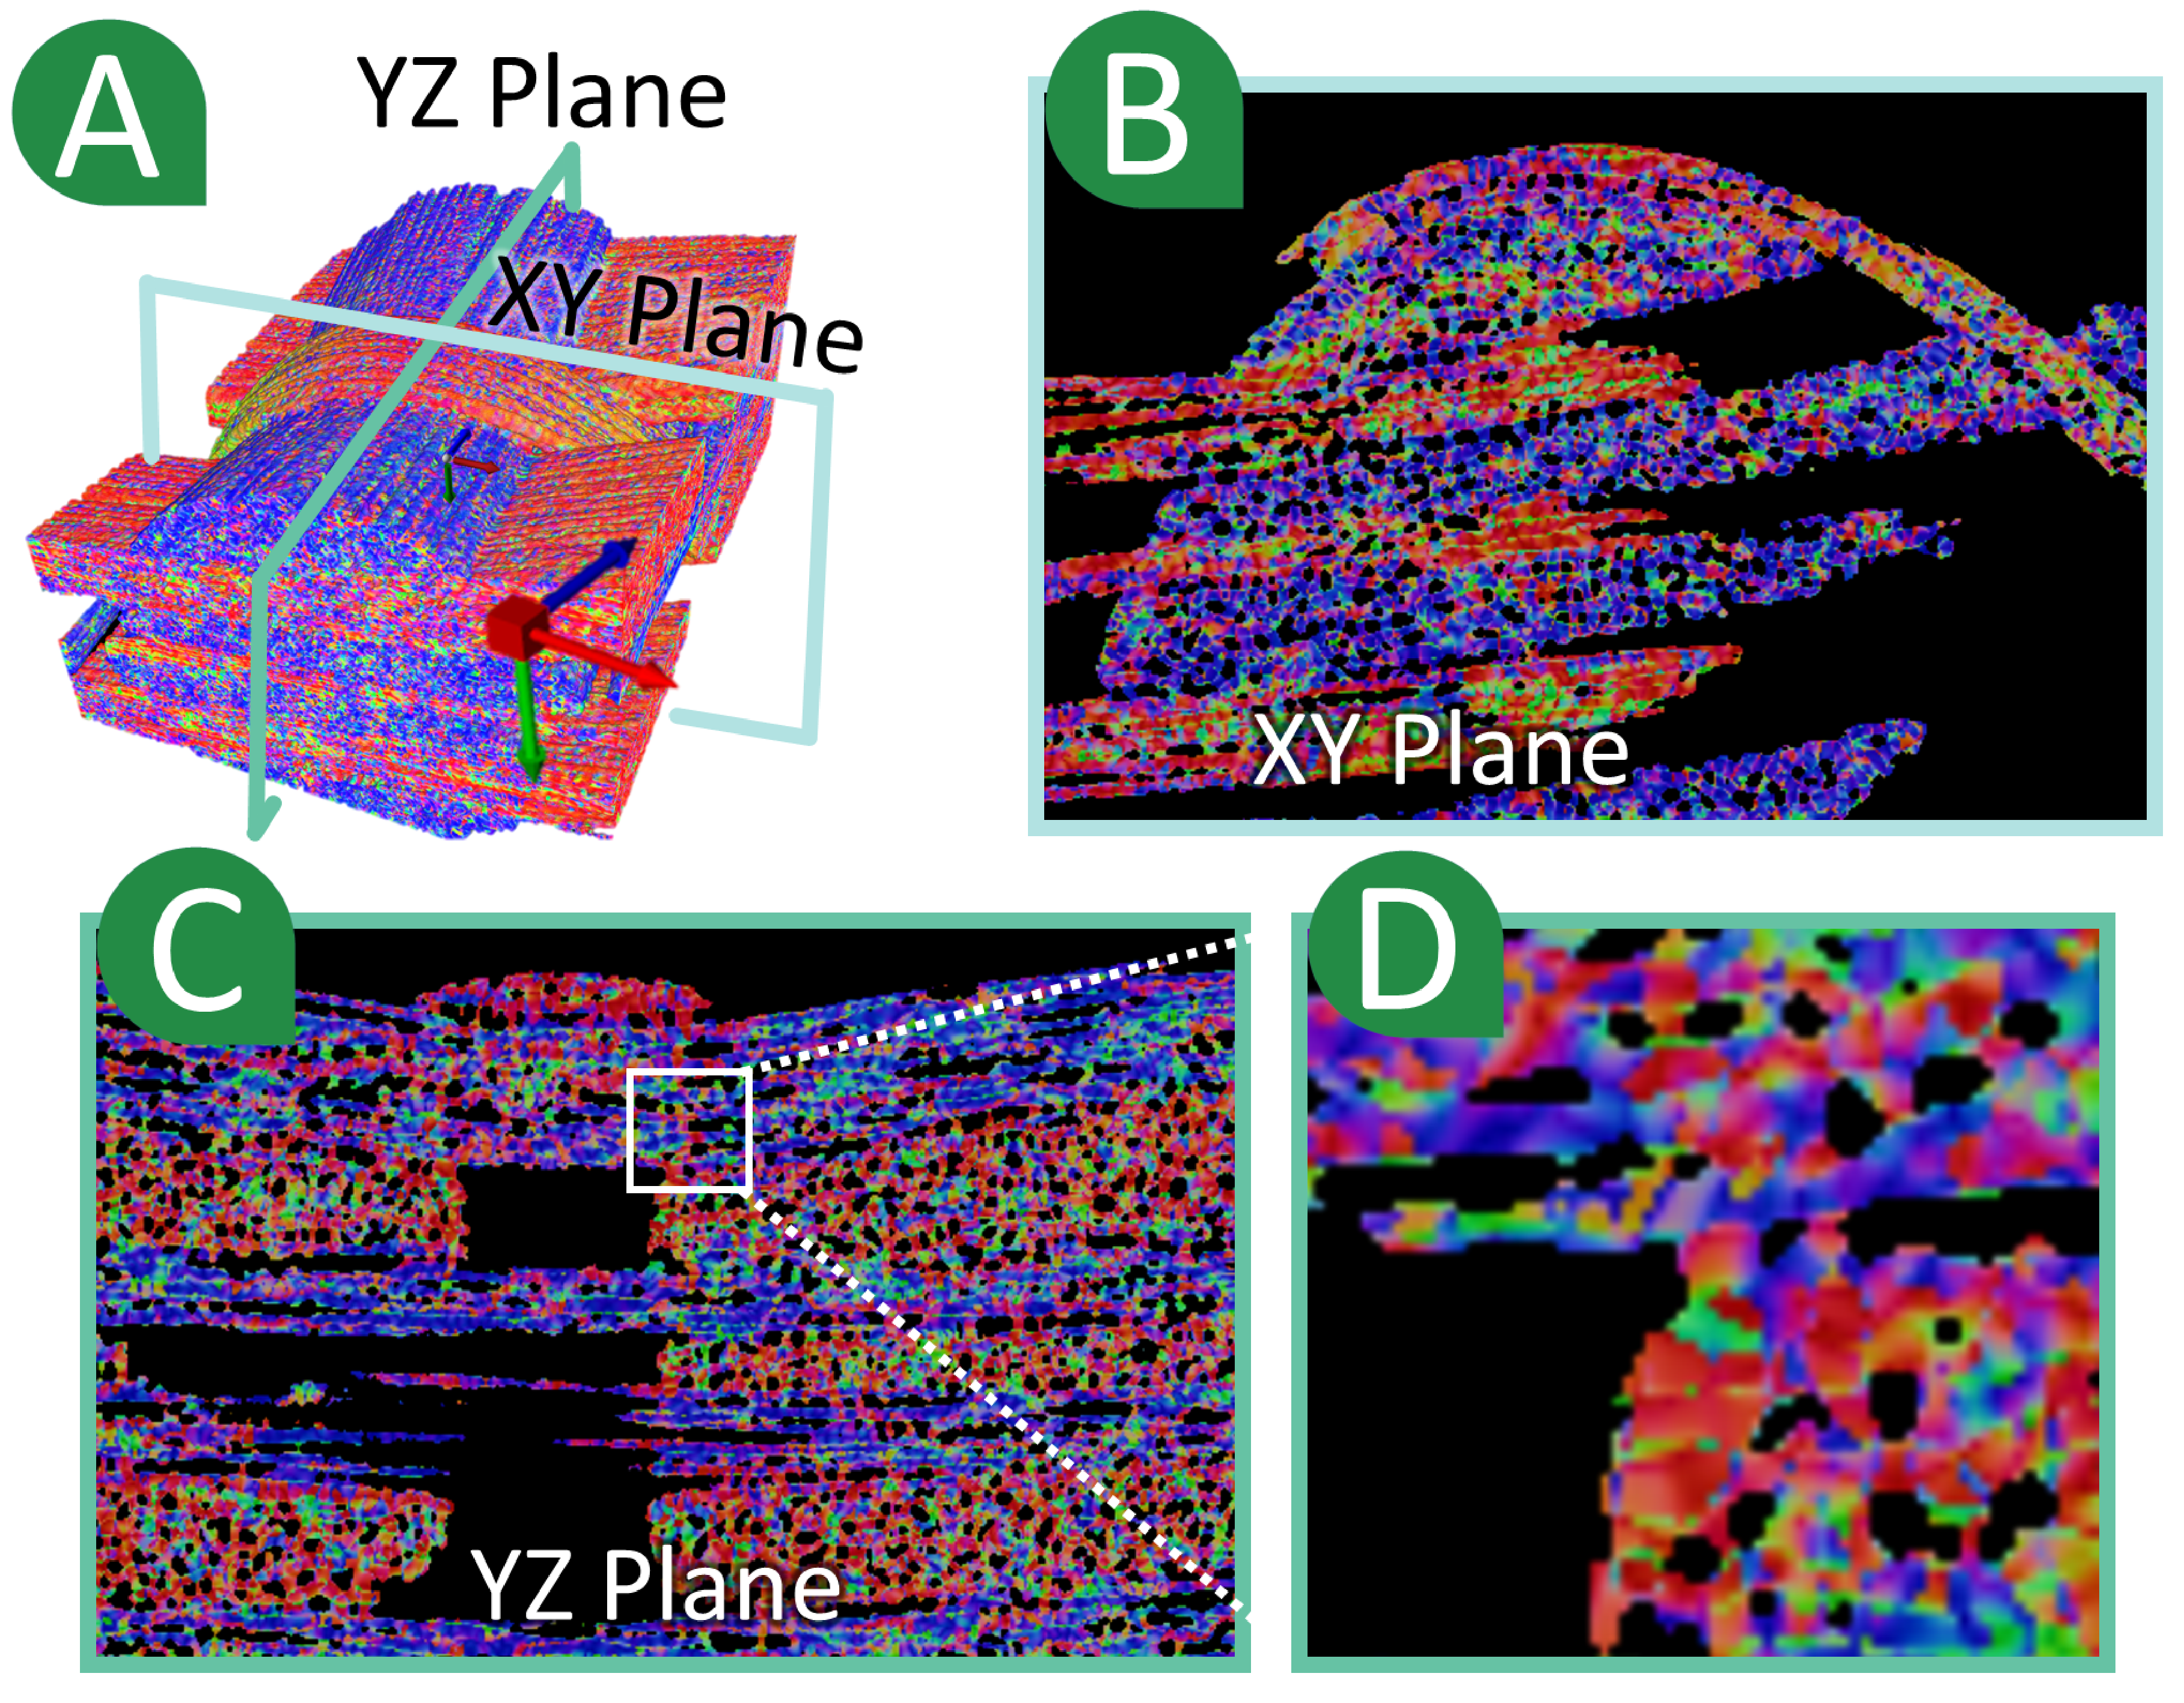
\includegraphics[width=\linewidth]{images/reliable_hessian2row.eps}
\caption{Reliable Hessians. (a) \mt colored according to the local orientation vector mapped to RGB color scale. (b,c) 2D slices along Z- and X- axis. (d) Magnified region marked in (c).}
\label{fig:reliable_hessian}
\vskip-0.2cm
\end{figure}
Figure~\ref{fig:reliable_hessian} shows the intermediate results of local orientation computation.
The principal direction represented as a unit vector has been mapped to RGB color space.
Figure~\ref{fig:reliable_hessian}\brac{a} shows the entire data set. 
Figure~\ref{fig:reliable_hessian}\brac{b},\brac{c} shows 2D slices along the Z- and X-axes respectively. Regions with X- and Z-axis local orientation show predominant red and blue color respectively.   Figure~\ref{fig:reliable_hessian}\brac{d} shows a magnified region of interest. The black regions within bundles are regions where the $R_H$ is less than the threshold and have unreliable local orientation. The bundles are also not uniformly colored as the Hessians and the corresponding principal directions are noisy.

We indicate some intrinsic differences between DTI and our XCT data. Fiber traces can be generated in DTI using a standard fiber tracking algorithms following the principal direction of diffusion by employing a fourth order Runge-Kutta method~\cite{Brun2003}. The principal direction based on the Hessian matrix works best when the tubular structures in the data are well separated from the background. This is not the case for our data. The local orientations at each voxel are inherently noisier.
\subsection{\mt Properties}\label{subsec:mt_properties}
Conventional integral curve based techniques cannot be directly used to extract fiber bundle traces from reliable Hessians because of the spurious nature of the Hessian based local orientations.
Thus instead of building fiber traces, we define an abstract representation of the fibers.
We start from two key assumptions on the data, specifically ``local orientation" and ``connectivity", while taking into account the adverse effects of noise and low resolution.

This is achieved by interpreting the underlying geometric structure of the fibers as a set of connected cylinders. 
Hence, we formulate \mt as a coarse and simple approximation of integral curves. In the form of a continuous chain of cylindrical tubes in $\mathbb{R}^3$. \mt traverse the fiber bundles embedded in the original data. Extending the intuition developed above, 
we devise the following \textit{properties} that the \mt share;
\begin{enumerate}[noitemsep,nolistsep]
	\item{\mt are associated with a continuous set of cylinders.}
	\item{\mt are associated with a start point at a grid vertex.}
	\item{Individual cylinders in \mt have constant lengths, radii, and start points (which are also grid's vertices).}
	\item{Individual cylinders in \mt (except the first one) are connected to their previous cylinders at their start point.}
	\item{Individual cylinders are parallel to the local orientation vector at their start points.}
\end{enumerate} 

\subsection{\mt Generation}\label{subsec:mt_generation}

\begin{figure}[t]
\begin{center}
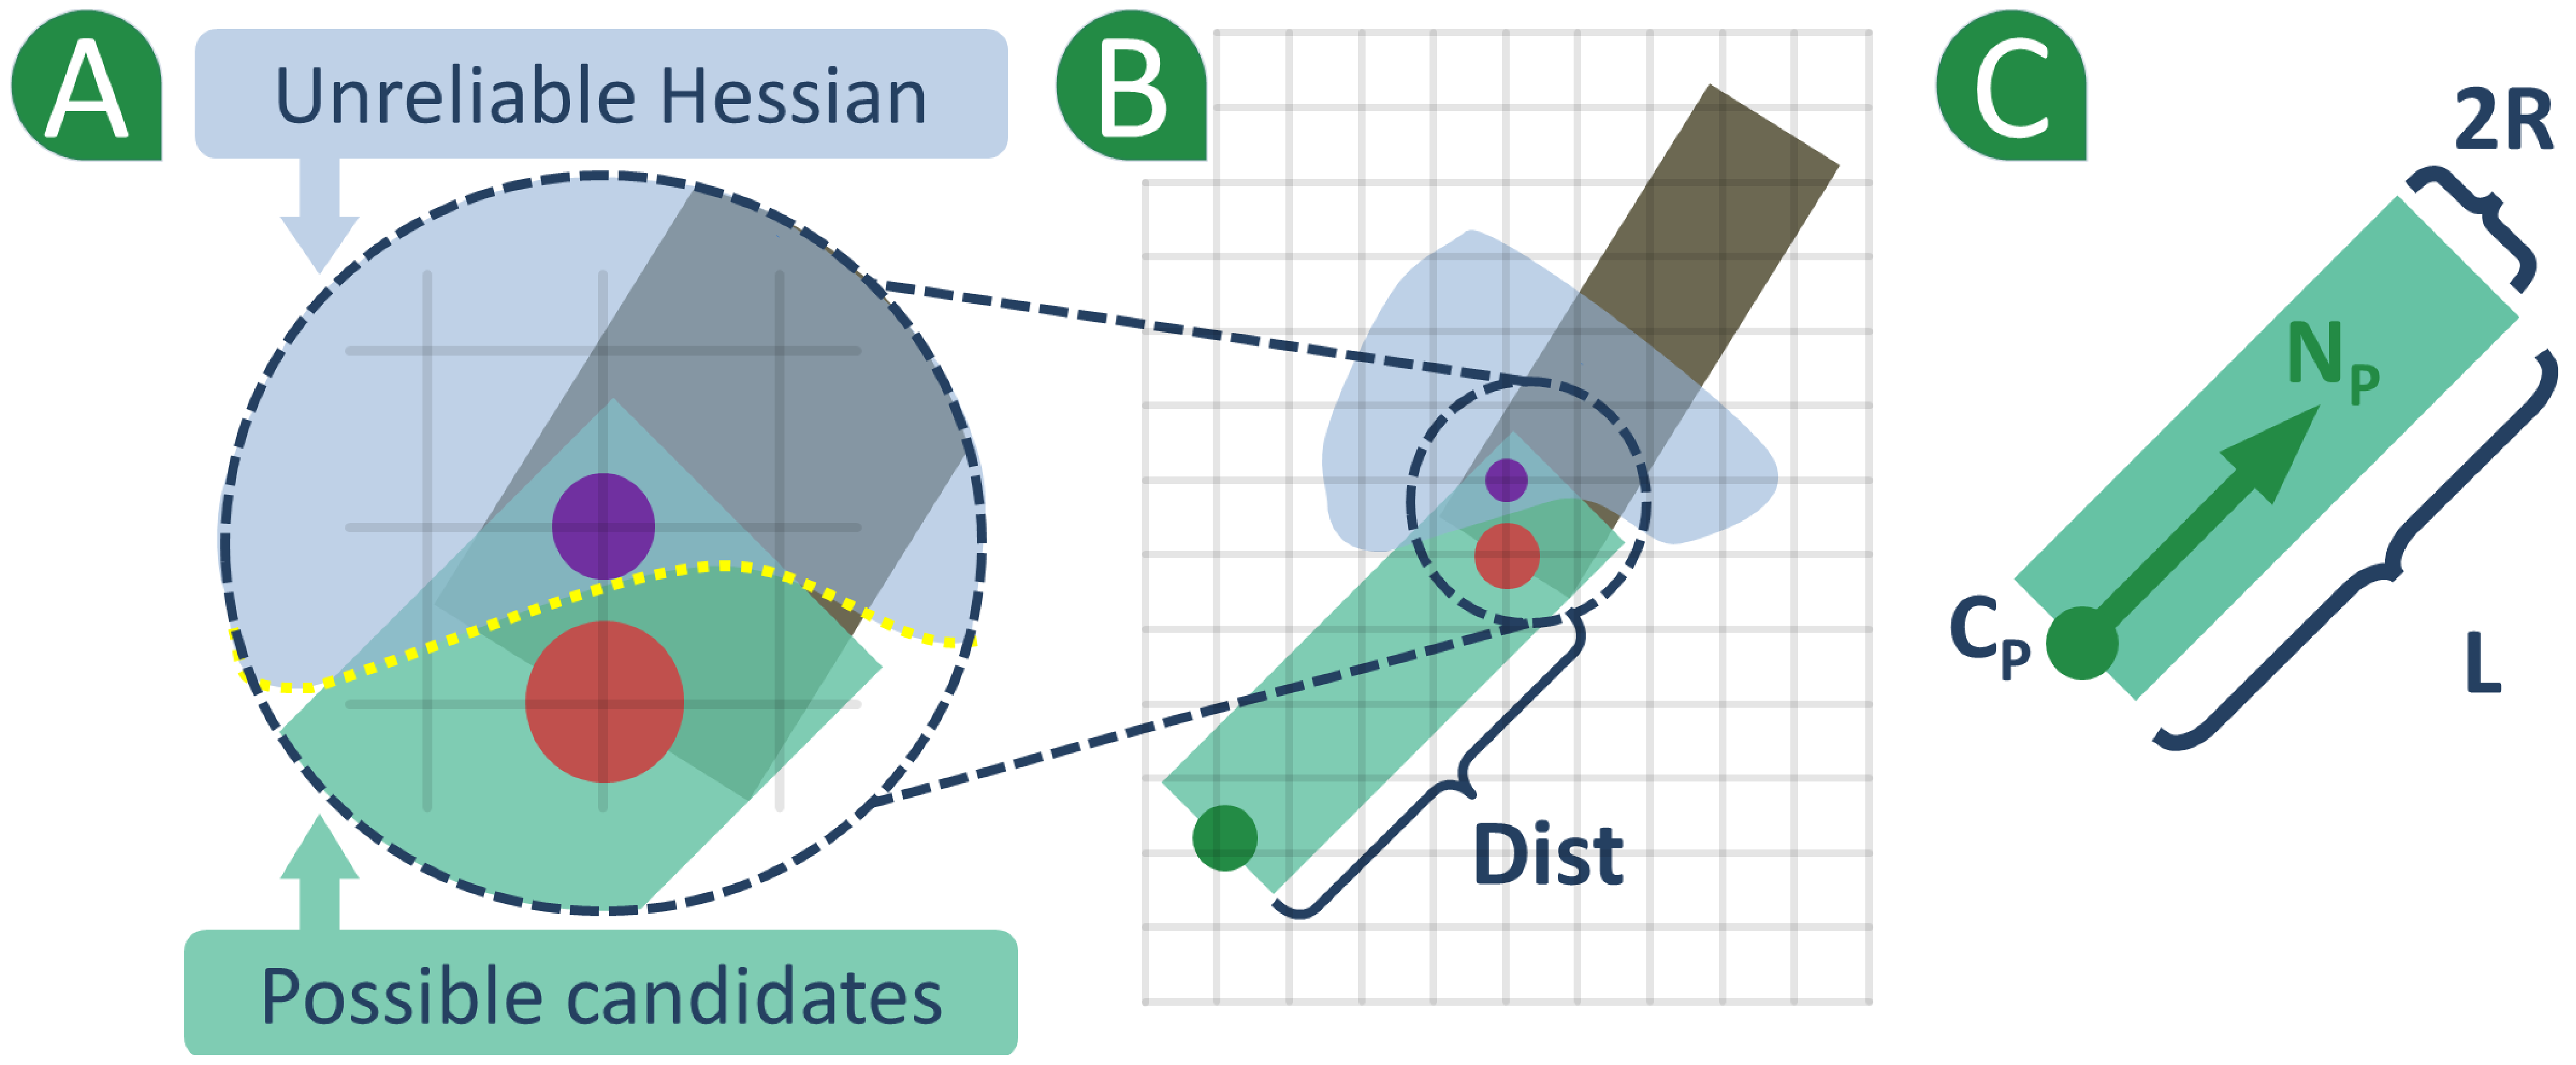
\includegraphics[ width=\linewidth]{images/mt_gen.eps}
\end{center}
\caption{MetaTracts generation. (b) \mt generation process. (a) Magnified region in (b). (c) Individual MetaTract cylinder. }
\label{fig:algo}
\end{figure}
In this section we detail the process of generating MetaTracts. Here we explain the process in  $\mathbb{R}^2$, the procedure extends to  $\mathbb{R}^3$ trivially. 
The output of the last (reliable Hessian) stage is input to the current step. In $\mathbb{R}^2$, each grid location is associated with a unit vector (representing the local orientation) and a reliability measure $R_H$[0,1]. Figure~\ref{fig:algo} shows some key features of MetaTracts. In Figure~\ref{fig:algo}\brac{a},\brac{b} the regions with unreliable Hessians are marked in blue. In $\mathbb{R}^2$ the individual components of \mt are rectangles. Figure~\ref{fig:algo}\brac{c} shows an individual rectangle, let the seed point associated with the MetaTract be grid point $C_{p}$ (property 2 in Sec.~\ref{subsec:mt_properties}). The local orientation at $C_p$ as computed in the reliable Hessian stage is $N_P$ and is given by the dark green arrow. The rectangle itself is of length $L$ and radius $R$ (properties 3 and 5 in Section~\ref{subsec:mt_properties}). 

We start with an individual rectangle with seed point $C_{p}$, local orientation $N_P$ and dimensions $L$, $R$. The set of grid vertices which are located within the rectangle (green region) in Figure~\ref{fig:algo}\brac{a},\brac{b} but are possible start points for the next cylinder. Among these we first discard the grid points which have unreliable Hessians (marked in blue). These set of grid points are called ``candidate vertices" and are potential start points. Based on the ``local orientation" and ``connectivity" assumptions on our data, we rank all the candidate points. The rank of each candidate point is based on the following characteristics.
\begin{itemize}[noitemsep,nolistsep]
\item \textit{Orientation similarity}: The local orientation of the start points ($N_p$) for the consecutive cylinders should be similar. 
\item \textit{Large distance}: The MetaTracts should traverse the data using as few cylinders as possible. Thus the distance between start point ($C_p$) of one cylinder and the start point for the next cylinder should be as large as possible. We measure the distance of each candidate vertex from $C_p$ by projecting the Euclidean distance between them onto $N_p$. For example, in Figure~\ref{fig:algo}\brac{b} the distance is measured as the Euclidean distance between the green and the orange vertices projected on to $N_p$. We refer to this perpendicular projection distance as \textit{`projected\_dist'}. 
\end{itemize}

We next define a ``priority" for each candidate vertex, based on the above characteristics. For each cylinder in a MetaTract, we put it's ``candidate vertices" in a priority queue based on Equation \ref{eqn:algo_1}.
\begin{equation}
Priority = \gamma_1 e^{(-angle^2 / \alpha^2)} + \gamma_2e^{(-projected\_dist^2 / \beta^2)}
\label{eqn:algo_1}
\end{equation}
$\gamma_1$, $\gamma_2$ are the  weights ($\mathbb{R}_{\ge 0}$)  which decide how the ``priority" depends on the affine combination of the two factors. For all our cases, we use $\gamma_1$ = $1 / 3 $ and $\gamma_2$ = $2 / 3$. In general, we suggest $\gamma_1 +\gamma_2 = 1 $ and $\gamma_1 \leq \gamma_2$. At each iteration, we pick the top element in the priority queue to generate the corresponding cylinder, and repeat the steps. Essentially, Equation~\ref{eqn:algo_1} selects a grid point which is farthest from the current start point and is going in a similar direction. This approach tackles noise/errors in local orientation better than integral curves by looking at multiple choices for vertex candidates and avoiding intra-cell interpolation in an already noisy environment. 

In Figure~\ref{fig:algo}\brac{b} the \textit{orange} grid vertex is selected next and process repeated. The \textit{purple} vertex is in a region of unreliable Hessian and is not selected even though it is further away from the seed point in terms of euclidean distance. \todo{If we generate \mt that have erroneous local orientations the size of the candidate vertex set will be small. This will create \mt of small length which are then removed.}

The \mt generated by the above procedure are shown in Figure~\ref{fig:metaTracts}. The \mt are colored with the mean orientation direction mapped to the RGB space. Figure~\ref{fig:metaTracts} also shows a single slice of YZ plane and the XY plane. \todo{Consistent orientation is a key intrinsic feature in our data which was not obvious from the original gray scale images, but becomes visually pronounced in generated \mt.}


Figure~\ref{fig:length_distribution} shows the MetaTracts of a particular bundle colored according to their individual length.\todo{ MetaTracts in a given fiber bundle may extend the full length of the bundle or have different lengths and partial overlaps.}

\begin{figure}[htb]
\centering
	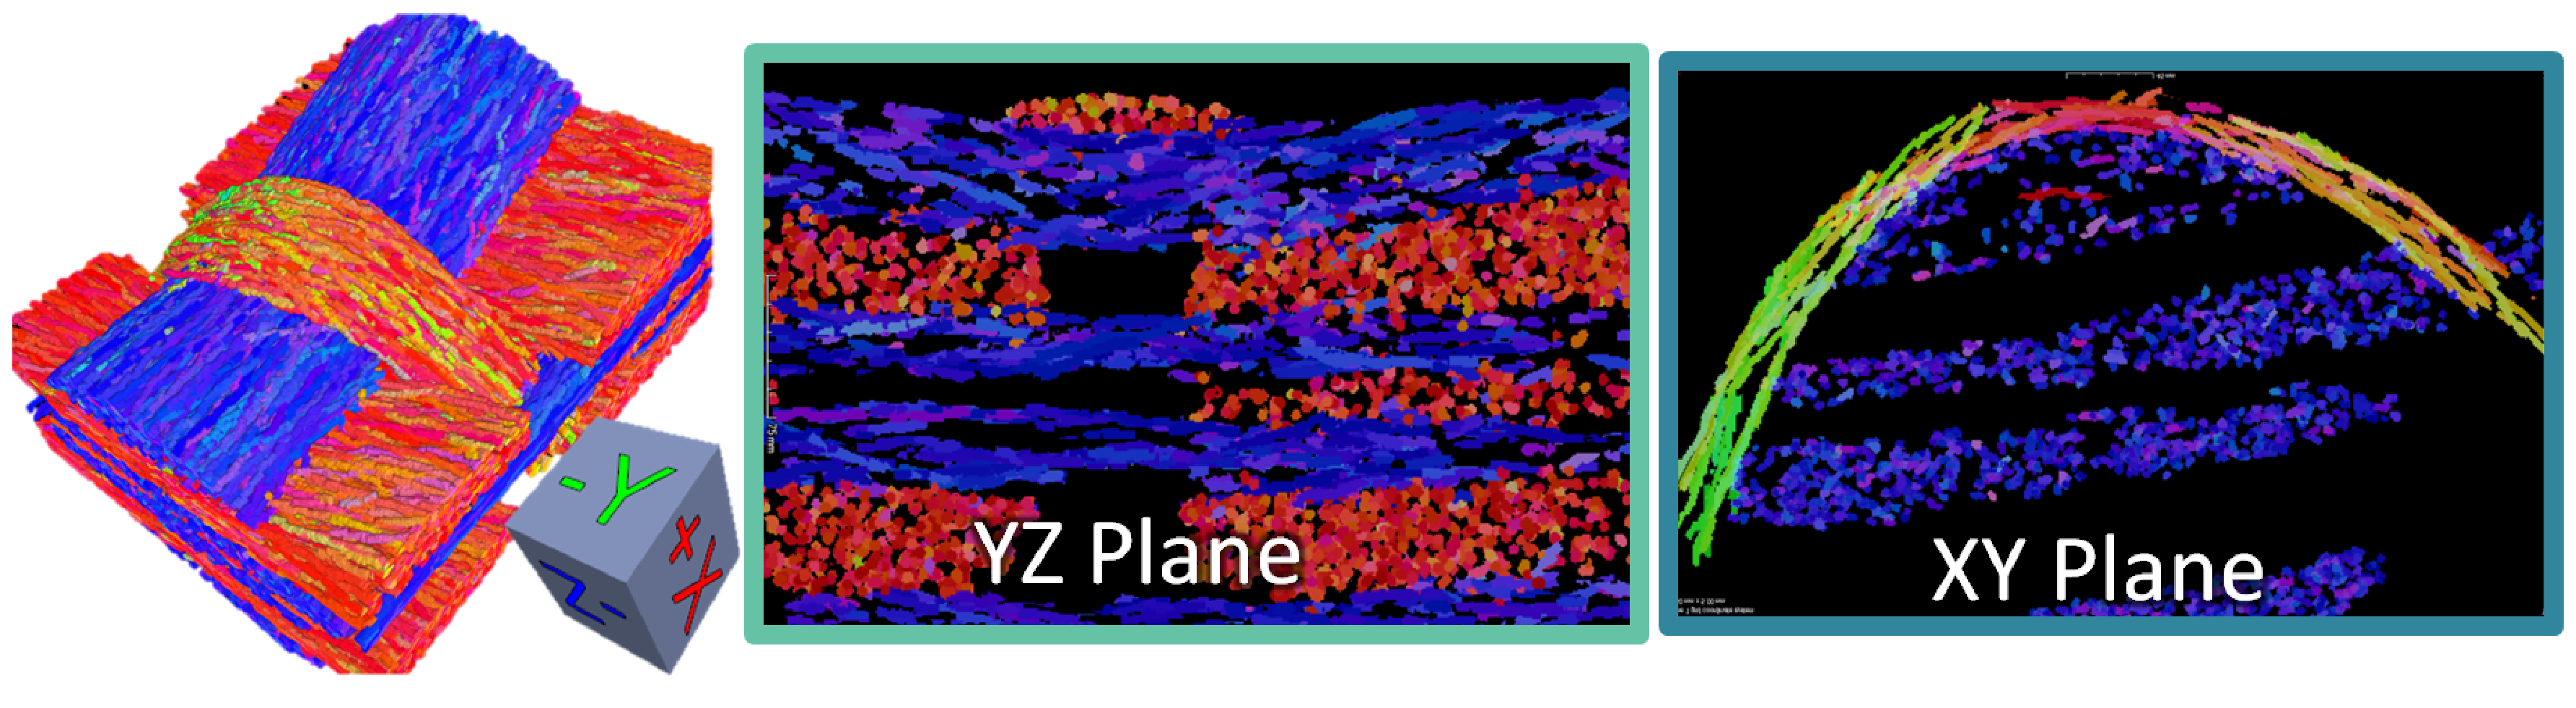
\includegraphics[width=\linewidth]{images/metaTracts.eps}
	\caption{(a) MetaTracts color-coded according to their mean orientations, along with slices of the YZ, XY-plane.}
	\label{fig:metaTracts}
\end{figure}

